\documentclass[12pt,letterpaper,onecolumn]{report} 
\usepackage[utf8]{inputenc}
\usepackage{amsmath}
\usepackage{amsfonts}
\usepackage{amssymb}
\usepackage{graphicx}
\usepackage[left=2cm,right=2cm,top=2cm,bottom=2cm]{geometry}
\author{Xia Liu}
\title{Latex workshop}   %can't have _ because it is in math mode, has to use between $$
\begin{document}
\maketitle %make title


%----------------------use othre latex file in this report-------
\chapter{Real First}
\label{chap:ActualFirst}

\noindent This is the chapter one content. You can have whatever you want 
continue writing, and continue and continue	

\noindent This is the last line of the file. %the file's name



%---------------chapter title-------------------article doesn't work with chapter
\chapter{First of many}
\label{chp:first}



\noindent I am standing at the front of the lecture \LaTeX . hall and showing what the hall i idont know what i am doing now sssssfffffsdfsdfa\\
%this is a comment where percentage symbol is used to make comment
\hrule % make a rule
\vspace{0.2cm} % add spacing or: /vsapce{24pt}
\hrule
\vspace{0.2cm} % add spacing 
\noindent my figure:


%------------------how to add, edit and ref figure in LaTeX-----------------------
\begin{figure}[!ht] % [!ht] ht puts images under the test
\centering
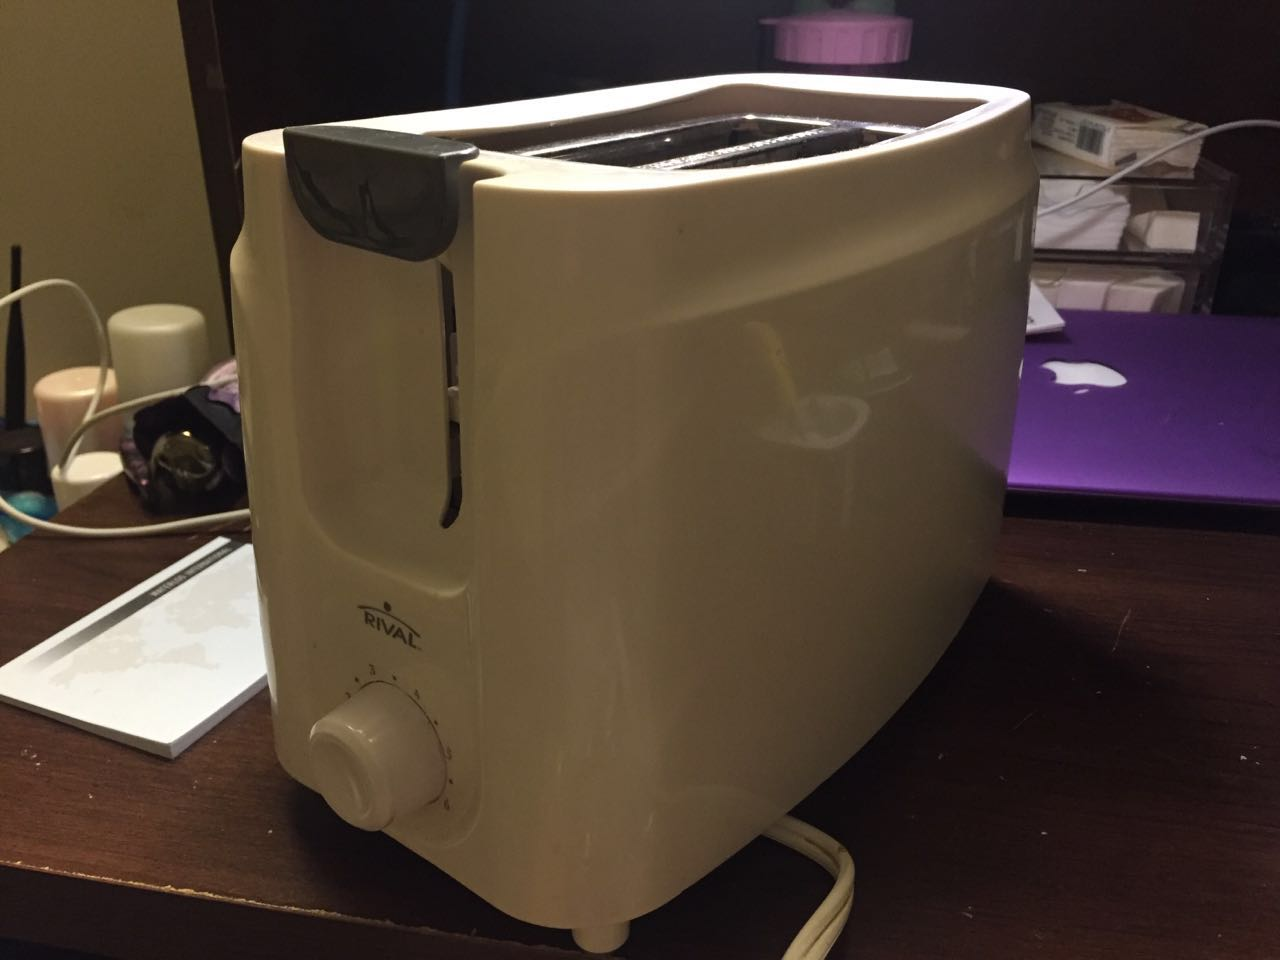
\includegraphics[width=\textwidth]{/home/xia/Pictures/toaster.jpg}
\caption{this is the first toaster}
\label{fig:gir} % is used to be referenced in the paragraph
\end{figure}

%----------------section---------------
\section{picture}
\label{sec:first}
\noindent I am standing at the front of the lecture \LaTeX . hall and showing what the hall i idont know what i am doing now sssssfffffsdfsdfa. this is the Figure \ref{fig:gir} some great toaster\\


\newpage % add new page
\section{picture2}
\label{sec:second}
\begin{figure}[!ht] % [!ht] ht puts images under the test
\centering
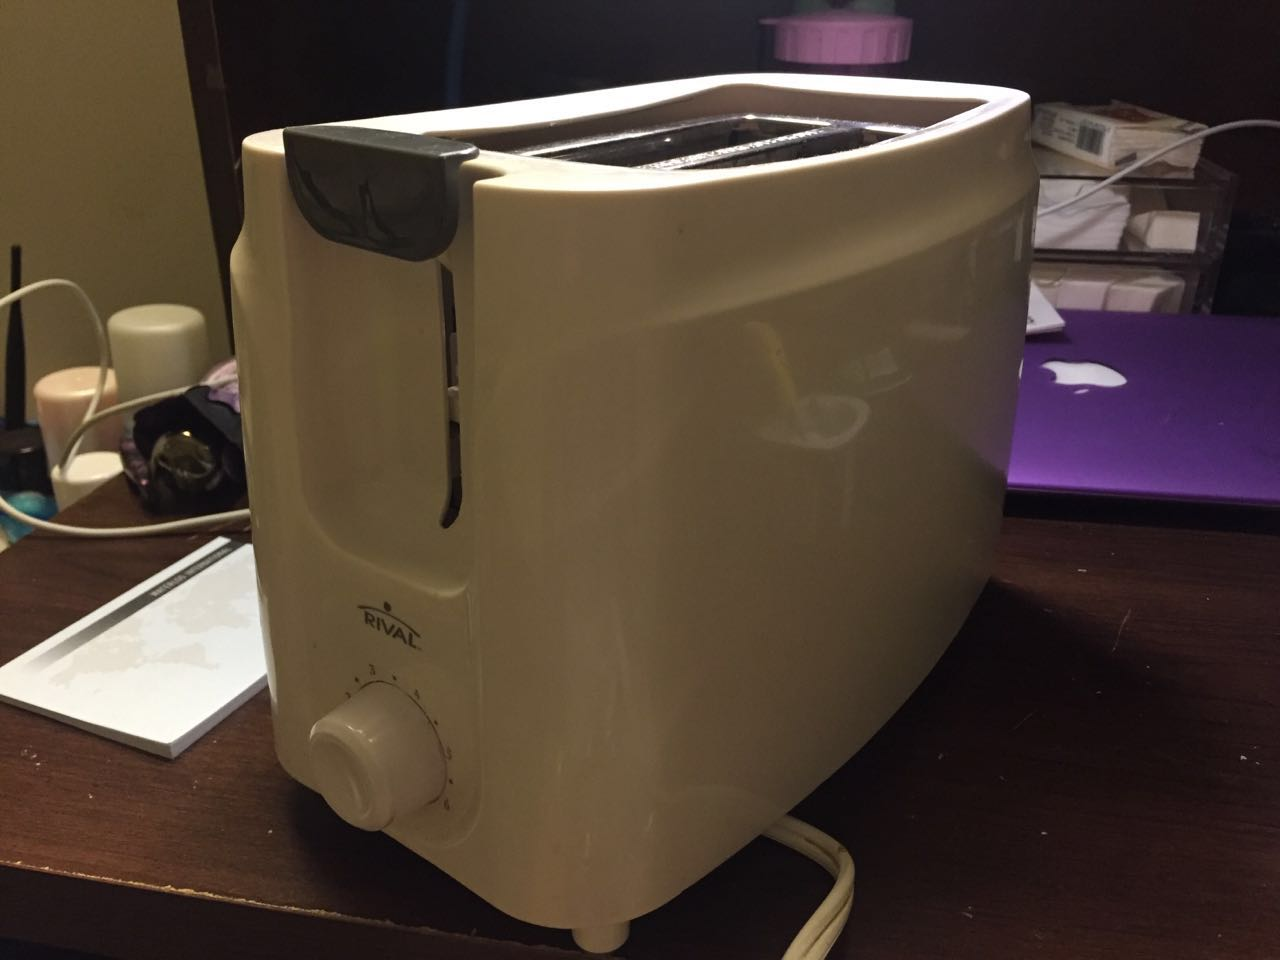
\includegraphics[scale=0.1]{/home/xia/Pictures/toaster.jpg}
\caption{This is a toaster} %add figure title
\label{it can be anything}
\end{figure}

\noindent I am standing at the front of the lecture \LaTeX . hall and showing what the hall i idont know what i am doing now. But not so bad, hahahaha, still need to do assignment  this is the Figure \ref{it can be anything} some great toaster\\

\subsection{picture2 sub}
\label{subsec:pic2sub}

\begin{figure}[!ht] % [!ht] ht puts images under the test
\caption{This is a toaster} %add figure title
\raggedright %the figure is put left side
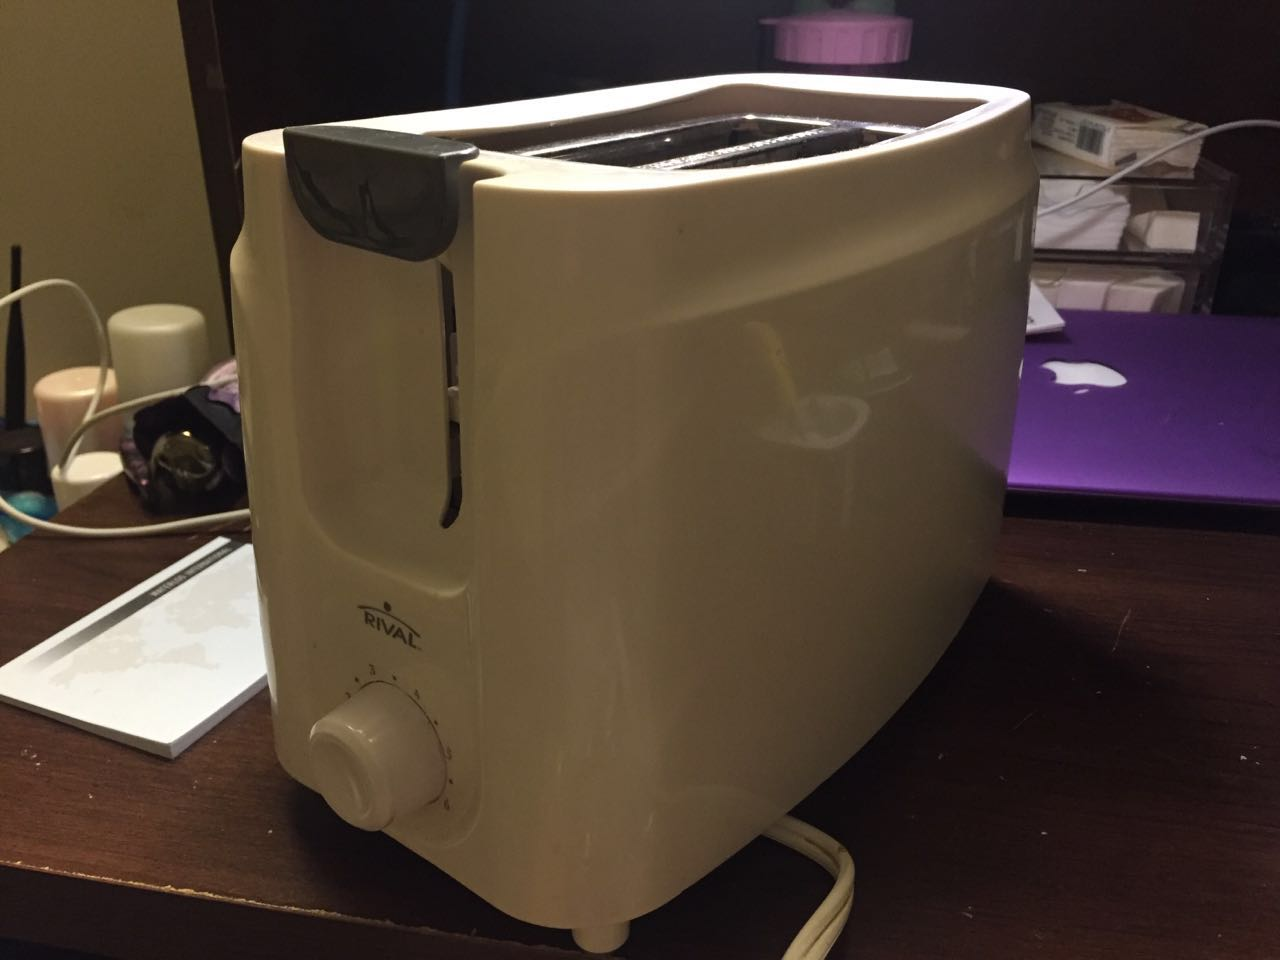
\includegraphics[scale=0.1]{/home/xia/Pictures/toaster.jpg}
\end{figure}

\chapter{Second of many}
\label{chap:second}
\noindent In the \ref{sec:first} we can see
%--------------------TABLE----------------------------------
\begin{table}[!ht]
\centering
\caption{This is mine information} % put title before the table
\begin{tabular}{|c|c |c |c| c |} %how many column.| means whether need vertical lines  c means center, r means right,l means left
\hline % means whetehr needs horizen lines
Name & Department & Student Number & Age &Race\\
\hline
\hline
Max & Math & 2000000 & 22 & ch\\
\hline
Max & Math & 2000000 & 22 & ch\\
\hline
Max & Math & 2000000 & 22 & ch\\
\hline
Max & Math & 2000000 & 22 & ch\\
\hline
Max & Math & 2000000 & 22 & ch\\
\hline
Max & Math & 2000000 & 22 & ch\\
\hline
\end{tabular}
\caption{This is mine information}
\label{tab:tab1}
\end{table}
Refer to figure \ref{fig:gir}, and table \ref{tab:tab1} % the first time, there is a ?, just repress F1



\newpage


%--------------------Equation------------------------
See equation \ref{equation:first}, this is the first simple example of equation
\begin{equation}
y=mx+b
\label{equation:first}
\end{equation}


See equation \ref{equation:second}, this is the second example of equation
\begin{equation}
y=\frac{top}{bottom}
\label{equation:second}
\end{equation}

% _ means for lowerbound, ^means for upperbound
See equation \ref{equation:third}, this is the third example of equation
\begin{equation}
\int e^x dx
=\int_{lowerbound}^{42} dx = 3754
\label{equation:third}
\end{equation}


See equation \ref{equation:forth}, this is the fourth example of equation. Putting = between \&, to make = in each line can be aligned, every $\setminus\setminus$ gives a new line number, $\setminus nonumber$ means no line number at the end of the line
\begin{eqnarray} %have multiple equations
y&=&mx+b\nonumber \\
&=&\frac{top}{botton}\nonumber	\\
\label{equation:forth}
&=&\int_{lowerbound}^{42} dx \\
=\lambda&=& 3754\\
\label{equation:five}
\end{eqnarray}


This sentence shows how to put an equation $\setminus\setminus$ like $\frac{top}{bottom} $ in text. 
Lowercase $\alpha$ and Uppercase $\Lambda \Gamma$. You can't have uppercase $\alpha$ and $\beta$ by using Alpha and Beta, because their uppercase formats are as same as A and B \cite{Terry2013}. %F6, F11,F6,F1 trytrytrytrytry
This is another reference according to this articles\cite{Lamport2001}.



%------------------Bibliography----------
%first, use mendeley, put all used articles into it and export a Bib.bib file(name can be changed, used in bibliopgraphy).  When to use it, do: \cite{x} x is the context in .bib after @arctile{
%You can create your own .bib file as long as follow the format
\medskip
\bibliographystyle{unsrt}
\bibliography{Bib}




\end{document}
